\documentclass[11pt,a4paper,landscape]{article}
\usepackage[margin=1.15cm]{geometry}
\usepackage{fontspec}
\IfFontExistsTF{Times New Roman}{\setmainfont{Times New Roman}}{\setmainfont{TeX Gyre Termes}}
\usepackage{xcolor}
\usepackage{tikz}
\usetikzlibrary{arrows.meta,calc}
\usepackage{amsmath}
\pagestyle{empty}
\setlength{\parindent}{0pt}

\definecolor{inputblue}{HTML}{DCEBFF}
\definecolor{featurecyan}{HTML}{DFF5F4}
\definecolor{regimegreen}{HTML}{DDF5E3}
\definecolor{globalorange}{HTML}{FDE7C8}
\definecolor{expertgold}{HTML}{FFF1C9}
\definecolor{blendpurple}{HTML}{E9DDF8}
\definecolor{outred}{HTML}{FADBDD}
\definecolor{linegray}{HTML}{425466}
\definecolor{titleblue}{HTML}{1F4E79}

\tikzset{
  >={Latex[length=3mm,width=2mm]},
  line/.style={draw=linegray, -Latex, line width=0.9pt},
  dashedline/.style={draw=linegray, -Latex, line width=0.82pt, dashed},
  panel/.style={draw=linegray, rounded corners=2.6mm, line width=0.7pt},
  box/.style={
    draw=linegray,
    rounded corners=1.8mm,
    align=center,
    font=\scriptsize,
    inner sep=3.4pt,
    minimum height=10mm
  }
}

\begin{document}

\begin{center}
{\LARGE\bfseries\color{titleblue} Sơ đồ tổng quan mô hình \texttt{anfis\_fuzzy\_regime\_hybrid.py}}\\[0.35em]
{\large Pipeline: OHLC features $\rightarrow$ fuzzy regime hybrid $\rightarrow$ blend/gating}
\end{center}

\begin{center}
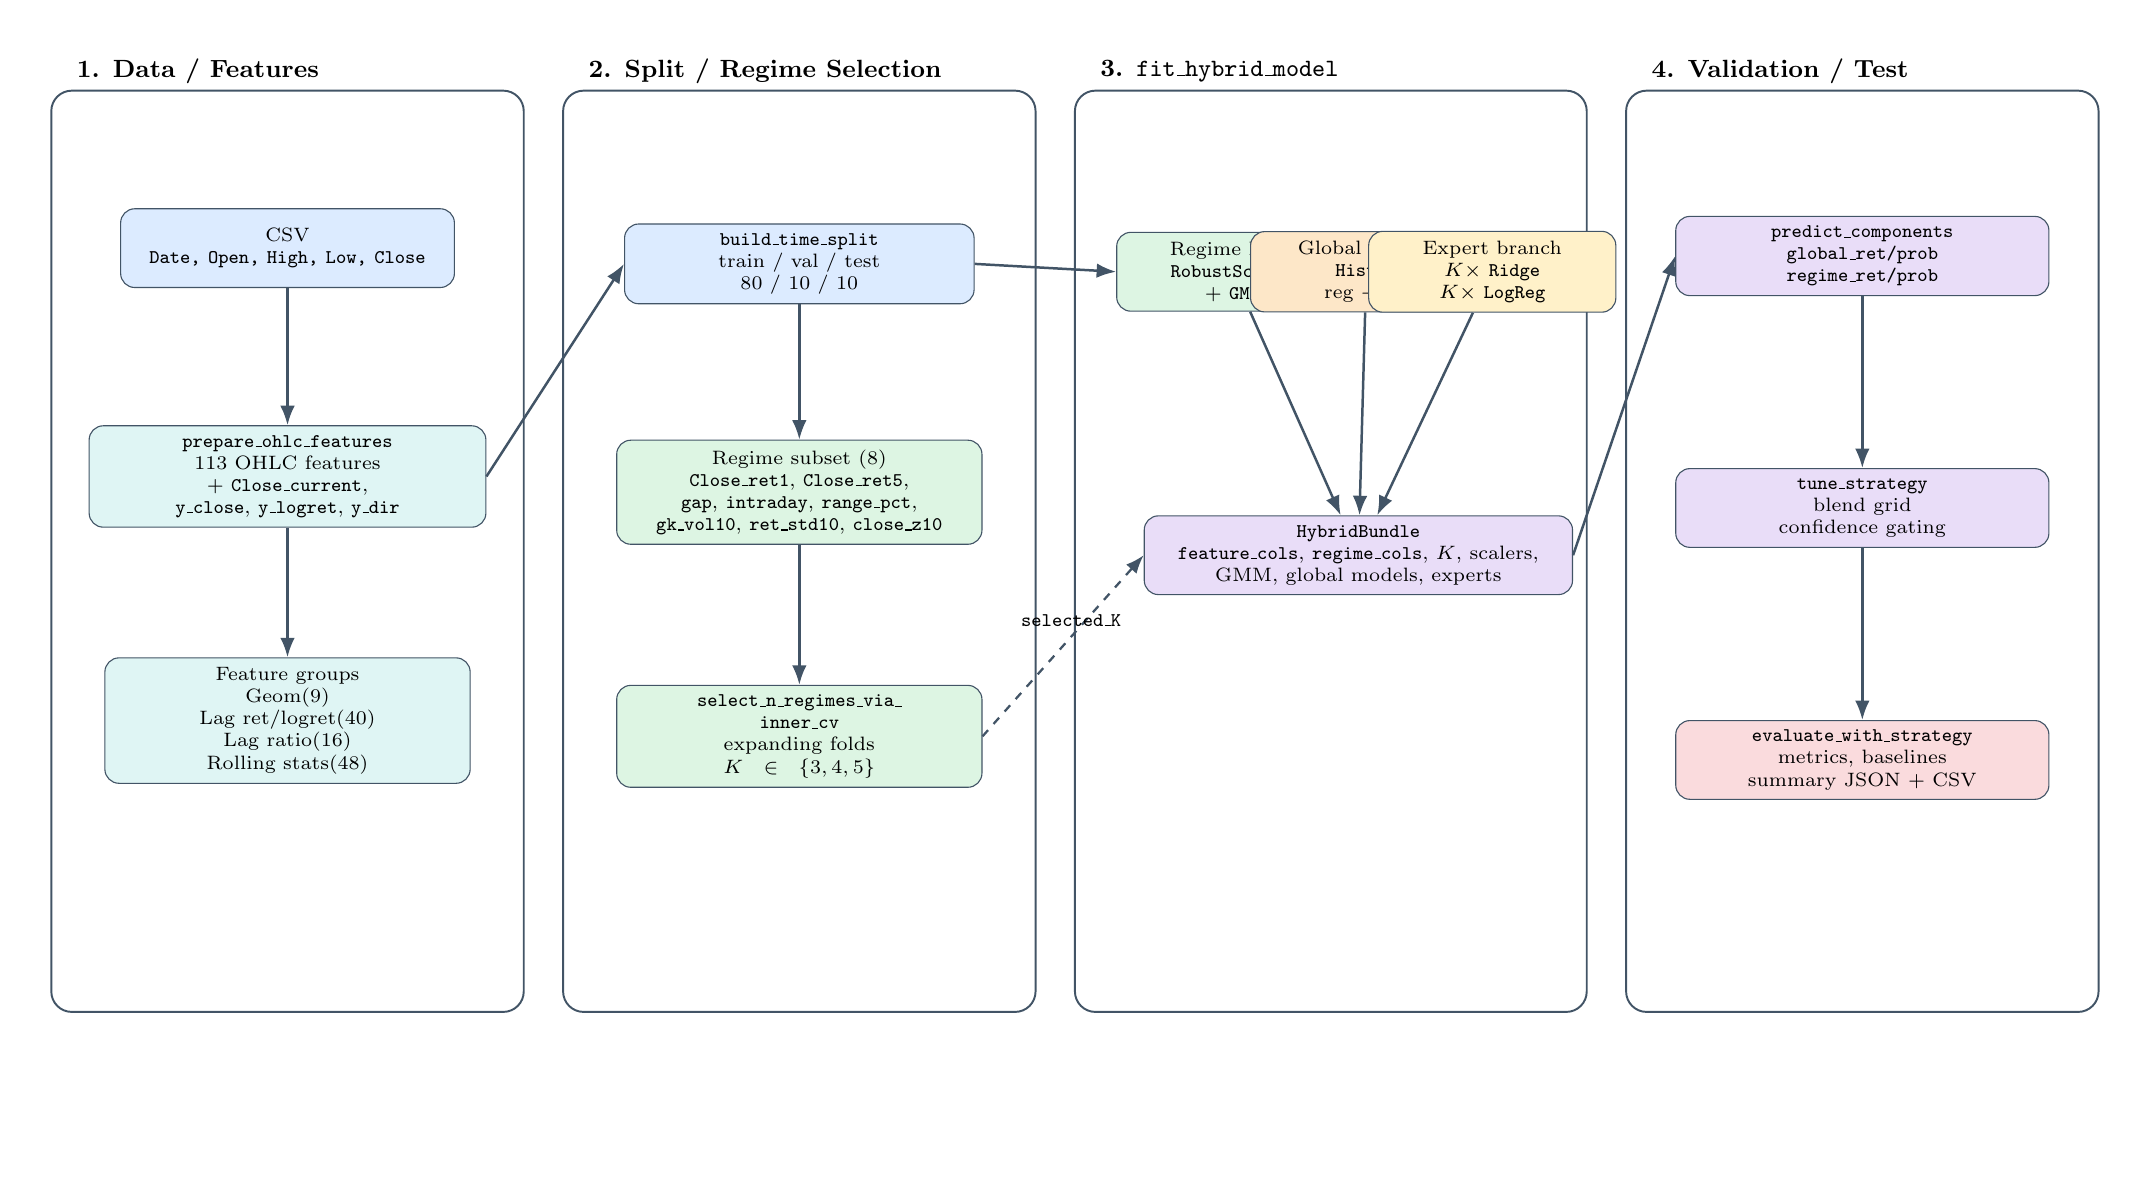
\begin{tikzpicture}[x=1cm,y=1cm]
  \path[use as bounding box] (0,0) rectangle (26.6,14.5);

  \draw[panel] (0.3,2.0) rectangle (6.3,13.7);
  \draw[panel] (6.8,2.0) rectangle (12.8,13.7);
  \draw[panel] (13.3,2.0) rectangle (19.8,13.7);
  \draw[panel] (20.3,2.0) rectangle (26.3,13.7);

  \node[anchor=west, font=\bfseries\small] at (0.5,13.95) {1. Data / Features};
  \node[anchor=west, font=\bfseries\small] at (7.0,13.95) {2. Split / Regime Selection};
  \node[anchor=west, font=\bfseries\small] at (13.5,13.95) {3. \texttt{fit\_hybrid\_model}};
  \node[anchor=west, font=\bfseries\small] at (20.5,13.95) {4. Validation / Test};

  \node[box, fill=inputblue, text width=4.0cm] (csv) at (3.3,11.7)
    {CSV\\\texttt{Date, Open, High, Low, Close}};
  \node[box, fill=featurecyan, text width=4.8cm] (prep) at (3.3,8.8)
    {\texttt{prepare\_ohlc\_features}\\113 OHLC features\\+\ \texttt{Close\_current}, \texttt{y\_close}, \texttt{y\_logret}, \texttt{y\_dir}};
  \node[box, fill=featurecyan, text width=4.4cm] (featgroups) at (3.3,5.7)
    {Feature groups\\Geom(9)\\Lag ret/logret(40)\\Lag ratio(16)\\Rolling stats(48)};

  \node[box, fill=inputblue, text width=4.2cm] (split) at (9.8,11.5)
    {\texttt{build\_time\_split}\\train / val / test\\80 / 10 / 10};
  \node[box, fill=regimegreen, text width=4.4cm] (subset) at (9.8,8.6)
    {Regime subset (8)\\\texttt{Close\_ret1}, \texttt{Close\_ret5}, \texttt{gap}, \texttt{intraday}, \texttt{range\_pct}, \texttt{gk\_vol10}, \texttt{ret\_std10}, \texttt{close\_z10}};
  \node[box, fill=regimegreen, text width=4.4cm] (innercv) at (9.8,5.5)
    {\texttt{select\_n\_regimes\_via\_}\\\texttt{inner\_cv}\\expanding folds\\$K \in \{3,4,5\}$};

  \node[box, fill=regimegreen, text width=2.7cm] (gmm) at (15.3,11.4)
    {Regime layer\\\texttt{RobustScaler}\\+\ \texttt{GMM}};
  \node[box, fill=globalorange, text width=2.7cm] (global) at (17.0,11.4)
    {Global branch\\\texttt{HistGB}\\reg + clf};
  \node[box, fill=expertgold, text width=2.9cm] (experts) at (18.6,11.4)
    {Expert branch\\$K \times$ \texttt{Ridge}\\$K \times$ \texttt{LogReg}};
  \node[box, fill=blendpurple, text width=5.2cm] (bundle) at (16.9,7.8)
    {\texttt{HybridBundle}\\\texttt{feature\_cols}, \texttt{regime\_cols}, $K$, scalers, GMM, global models, experts};

  \node[box, fill=blendpurple, text width=4.5cm] (predict) at (23.3,11.6)
    {\texttt{predict\_components}\\\texttt{global\_ret/prob}\\\texttt{regime\_ret/prob}};
  \node[box, fill=blendpurple, text width=4.5cm] (tune) at (23.3,8.4)
    {\texttt{tune\_strategy}\\blend grid\\confidence gating};
  \node[box, fill=outred, text width=4.5cm] (eval) at (23.3,5.2)
    {\texttt{evaluate\_with\_strategy}\\metrics, baselines\\summary JSON + CSV};

  \draw[line] (csv) -- (prep);
  \draw[line] (prep) -- (featgroups);
  \draw[line] (prep.east) -- (split.west);
  \draw[line] (split) -- (subset);
  \draw[line] (subset) -- (innercv);
  \draw[line] (split.east) -- (gmm.west);
  \draw[dashedline] (innercv.east) -- node[pos=0.55, above, font=\scriptsize] {\texttt{selected\_K}} (bundle.west);
  \draw[line] (gmm) -- (bundle);
  \draw[line] (global) -- (bundle);
  \draw[line] (experts) -- (bundle);
  \draw[line] (bundle.east) -- (predict.west);
  \draw[line] (predict) -- (tune);
  \draw[line] (tune) -- (eval);
\end{tikzpicture}
\end{center}

\newpage

\begin{center}
{\LARGE\bfseries\color{titleblue} Sơ đồ chi tiết 1: feature engineering và chọn số regime}\\[0.35em]
{\large \texttt{prepare\_ohlc\_features} + \texttt{build\_time\_split} + \texttt{select\_n\_regimes\_via\_inner\_cv}}
\end{center}

\begin{center}
\begin{tikzpicture}[x=1cm,y=1cm]
  \path[use as bounding box] (0,0) rectangle (26.6,14.5);

  \draw[panel] (0.3,8.1) rectangle (26.3,13.7);
  \draw[panel] (0.3,1.0) rectangle (26.3,6.9);

  \node[anchor=west, font=\bfseries\small] at (0.5,13.95) {A. \texttt{prepare\_ohlc\_features}};
  \node[anchor=west, font=\bfseries\small] at (0.5,7.15) {B. Split thời gian và chọn \texttt{n\_regimes}};

  \node[box, fill=inputblue, text width=2.8cm] (raw) at (1.8,10.9)
    {Raw OHLC\\CSV};
  \node[box, fill=inputblue, text width=3.2cm] (clean) at (5.2,10.9)
    {Parse \texttt{Date}\\sort, filter\\numeric, drop OHLC-NaN};
  \node[box, fill=featurecyan, text width=2.9cm] (geom) at (8.7,11.9)
    {Geom (9)\\gap\\intraday\\range\\wick\\pos};
  \node[box, fill=featurecyan, text width=2.9cm] (lagret) at (12.1,11.9)
    {Lag ret/logret (40)\\OHLC\\lags 1,2,3,5,10};
  \node[box, fill=featurecyan, text width=2.7cm] (lagratio) at (15.3,11.9)
    {Lag ratio (16)\\OHLC\\lags 1,2,3,5};
  \node[box, fill=featurecyan, text width=3.6cm] (rolling) at (19.3,11.9)
    {Rolling stats (48)\\\texttt{close\_z}\\ret mean/std/skew\\gk/park vol\\gap/body/range\\up/high/low break};
  \node[box, fill=featurecyan, text width=3.2cm] (matrix) at (23.5,11.8)
    {Feature matrix $X$\\113 columns};
  \node[box, fill=featurecyan, text width=3.2cm] (targets) at (23.5,9.2)
    {Targets\\\texttt{Close\_current}\\\texttt{y\_close}\\\texttt{y\_logret}\\\texttt{y\_dir}};

  \node[box, fill=inputblue, text width=3.2cm] (full) at (2.2,4.1)
    {Engineered DF\\113 features};
  \node[box, fill=inputblue, text width=3.4cm] (timesplit) at (6.5,4.1)
    {\texttt{build\_time\_split}\\train / val / test\\80 / 10 / 10};
  \node[box, fill=inputblue, text width=3.2cm] (mins) at (6.5,2.1)
    {\texttt{MIN\_TRAIN}=400\\\texttt{MIN\_VAL}=60\\\texttt{MIN\_TEST}=60};
  \node[box, fill=regimegreen, text width=3.4cm] (regcols) at (11.0,4.9)
    {\texttt{regime\_cols}\\8 features};
  \node[box, fill=regimegreen, text width=3.6cm] (folds) at (11.0,2.7)
    {\texttt{build\_expanding\_folds}\\train expands\\val slides forward};
  \node[box, fill=regimegreen, text width=4.2cm] (cv2) at (16.2,4.1)
    {\texttt{select\_n\_regimes\_via\_}\\\texttt{inner\_cv}\\fit on sub-train\\score on sub-val};
  \node[box, fill=blendpurple, text width=4.4cm] (score) at (21.6,4.1)
    {\texttt{score\_metrics}\\mean score across folds\\$\Rightarrow$ \texttt{selected\_K}};

  \coordinate (fanfeat) at (6.9,10.9);
  \draw[line] (raw) -- (clean);
  \draw[line] (clean.east) -- (fanfeat);
  \draw[line] (fanfeat) |- (geom.west);
  \draw[line] (fanfeat) |- (lagret.west);
  \draw[line] (fanfeat) |- (lagratio.west);
  \draw[line] (fanfeat) |- (rolling.west);
  \draw[line] (geom) -- (matrix);
  \draw[line] (lagret) -- (matrix);
  \draw[line] (lagratio) -- (matrix);
  \draw[line] (rolling) -- (matrix);
  \draw[line] (clean.east) -| (targets.west);

  \draw[line] (matrix.south) |- (full.north);
  \draw[dashedline] (targets.south) |- (full.north);
  \draw[line] (full) -- (timesplit);
  \draw[line] (timesplit) -- (regcols);
  \draw[line] (timesplit) -- (folds);
  \draw[line] (timesplit) -- (mins);
  \draw[line] (regcols) -- (cv2);
  \draw[line] (folds) -- (cv2);
  \draw[line] (cv2) -- (score);
\end{tikzpicture}
\end{center}

\newpage

\begin{center}
{\LARGE\bfseries\color{titleblue} Sơ đồ chi tiết 2: huấn luyện \texttt{HybridBundle}}\\[0.35em]
{\large \texttt{fit\_regime\_model} + \texttt{get\_memberships} + \texttt{fit\_hybrid\_model}}
\end{center}

\begin{center}
\begin{tikzpicture}[x=1cm,y=1cm]
  \path[use as bounding box] (0,0) rectangle (26.6,14.5);

  \draw[panel] (0.3,1.3) rectangle (5.1,13.7);
  \draw[panel] (5.6,1.3) rectangle (10.7,13.7);
  \draw[panel] (11.2,1.3) rectangle (16.4,13.7);
  \draw[panel] (16.9,1.3) rectangle (22.1,13.7);
  \draw[panel] (22.6,1.3) rectangle (26.3,13.7);

  \node[anchor=west, font=\bfseries\small] at (0.5,13.95) {A. Train targets};
  \node[anchor=west, font=\bfseries\small] at (5.8,13.95) {B. Regime layer};
  \node[anchor=west, font=\bfseries\small] at (11.4,13.95) {C. Global branch};
  \node[anchor=west, font=\bfseries\small] at (17.1,13.95) {D. Expert branch};
  \node[anchor=west, font=\bfseries\small] at (22.8,13.95) {E. Bundle};

  \node[box, fill=inputblue, text width=3.2cm] (train) at (2.7,11.8)
    {\texttt{split.train}};
  \node[box, fill=inputblue, text width=2.8cm] (xtrain) at (2.7,9.5)
    {\texttt{x\_train}\\$N \times 113$};
  \node[box, fill=inputblue, text width=2.8cm] (yret) at (2.7,7.2)
    {\texttt{y\_logret}};
  \node[box, fill=inputblue, text width=2.8cm] (ydir) at (2.7,4.9)
    {\texttt{y\_dir}};

  \node[box, fill=regimegreen, text width=3.0cm] (rinput) at (8.2,11.8)
    {\texttt{train[regime\_cols]}\\$N \times 8$};
  \node[box, fill=regimegreen, text width=3.0cm] (rscale) at (8.2,9.3)
    {\texttt{RobustScaler}};
  \node[box, fill=regimegreen, text width=3.0cm] (gmm2) at (8.2,6.8)
    {\texttt{GaussianMixture}\\diag / spherical};
  \node[box, fill=regimegreen, text width=3.2cm] (wtrain) at (8.2,4.3)
    {\texttt{memberships = W}\\$N \times K$};

  \node[box, fill=globalorange, text width=3.1cm] (xaug) at (13.8,11.6)
    {\texttt{x\_train\_aug}\\$[x\_train \mid W]$};
  \node[box, fill=globalorange, text width=3.1cm] (hgr) at (13.8,8.7)
    {\texttt{HistGBRegressor}\\$\rightarrow$ \texttt{global\_ret}};
  \node[box, fill=globalorange, text width=3.1cm] (hgc) at (13.8,5.8)
    {\texttt{HistGBClassifier}\\$\rightarrow$ \texttt{global\_prob}};

  \node[box, fill=expertgold, text width=3.2cm] (xscaled) at (19.5,11.6)
    {\texttt{expert\_scaler}\\\texttt{fit\_transform}\\\texttt{(x\_train)}};
  \node[box, fill=expertgold, text width=3.2cm] (weights) at (19.5,9.0)
    {For regime $k$\\\texttt{sample\_weight = W[:,k]}};
  \node[box, fill=expertgold, text width=3.2cm] (ridgek) at (19.5,6.4)
    {$K \times$ \texttt{Ridge}\\fit tới \texttt{y\_logret}};
  \node[box, fill=expertgold, text width=3.2cm] (logitk) at (19.5,3.8)
    {$K \times$ \texttt{LogReg}\\fit tới \texttt{y\_dir}};

  \node[box, fill=blendpurple, text width=3.0cm] (bundle2) at (24.4,8.2)
    {\texttt{HybridBundle}\\all trained state};

  \draw[line] (train) -- (xtrain);
  \draw[line] (train) -- (yret);
  \draw[line] (train) -- (ydir);

  \draw[line] (train.east) -- (rinput.west);
  \draw[line] (rinput) -- (rscale);
  \draw[line] (rscale) -- (gmm2);
  \draw[line] (gmm2) -- (wtrain);

  \draw[line] (xtrain.east) -- (xaug.west);
  \draw[dashedline] (wtrain.east) -| (xaug.south);
  \draw[line] (xaug) -- (hgr);
  \draw[line] (xaug) -- (hgc);

  \draw[line] (xtrain.east) |- (xscaled.west);
  \draw[dashedline] (wtrain.east) |- (weights.west);
  \draw[line] (xscaled) -- (weights);
  \draw[line] (weights) -- (ridgek);
  \draw[line] (weights) -- (logitk);
  \draw[dashedline] (yret.east) -| (ridgek.west);
  \draw[dashedline] (ydir.east) -| (logitk.west);

  \draw[line] (hgr.east) -- (bundle2.west);
  \draw[line] (hgc.east) -- (bundle2.west);
  \draw[line] (ridgek.east) -| (bundle2.south west);
  \draw[line] (logitk.east) -| (bundle2.south west);
  \draw[dashedline] (wtrain.east) -| (bundle2.west);
\end{tikzpicture}
\end{center}

\newpage

\begin{center}
{\LARGE\bfseries\color{titleblue} Sơ đồ chi tiết 3: suy luận, blend, gating, output}\\[0.35em]
{\large \texttt{predict\_components} + \texttt{blend\_predictions} + \texttt{tune\_strategy} + \texttt{evaluate\_with\_strategy}}
\end{center}

\begin{center}
\begin{tikzpicture}[x=1cm,y=1cm]
  \path[use as bounding box] (0,0) rectangle (26.6,14.5);

  \draw[panel] (0.3,1.6) rectangle (8.5,13.7);
  \draw[panel] (9.0,1.6) rectangle (17.6,13.7);
  \draw[panel] (18.1,1.6) rectangle (26.3,13.7);

  \node[anchor=west, font=\bfseries\small] at (0.5,13.95) {A. \texttt{predict\_components}};
  \node[anchor=west, font=\bfseries\small] at (9.2,13.95) {B. \texttt{tune\_strategy}};
  \node[anchor=west, font=\bfseries\small] at (18.3,13.95) {C. \texttt{evaluate\_with\_strategy}};

  \node[box, fill=inputblue, text width=3.2cm] (part) at (2.3,11.7)
    {\texttt{split.val} / \texttt{split.test}};
  \node[box, fill=regimegreen, text width=3.0cm] (mem2) at (5.8,11.7)
    {\texttt{memberships}\\\texttt{get\_memberships}};
  \node[box, fill=globalorange, text width=3.0cm] (gaug2) at (2.3,8.8)
    {\texttt{x\_aug}\\$[x \mid W]$};
  \node[box, fill=expertgold, text width=3.0cm] (xscaled2) at (5.8,8.8)
    {\texttt{x\_scaled}\\expert scaler};
  \node[box, fill=globalorange, text width=3.0cm] (gout) at (2.3,5.9)
    {\texttt{global\_ret}\\\texttt{global\_prob}};
  \node[box, fill=expertgold, text width=3.0cm] (emats) at (5.8,5.9)
    {\texttt{reg\_matrix}\\\texttt{clf\_matrix}};
  \node[box, fill=blendpurple, text width=4.2cm] (components) at (4.0,3.0)
    {\texttt{regime\_ret = W * reg\_matrix}\\\texttt{regime\_prob = W * clf\_matrix}\\components dict};

  \node[box, fill=blendpurple, text width=3.8cm] (blend) at (11.3,11.7)
    {\texttt{blend\_predictions}\\$r = \alpha_r r_{reg} + (1-\alpha_r) r_{glob}$\\$p = \alpha_p p_{reg} + (1-\alpha_p) p_{glob}$};
  \node[box, fill=blendpurple, text width=3.8cm] (grid) at (15.2,11.7)
    {Grid\\$\alpha_r,\alpha_p \in \{0.25,0.5,0.75\}$\\shrink $\in \{0.9,1.0,1.1\}$\\conf $\in \{0,\dots,0.4\}$\\dir $\in \{0.45,0.5,0.55\}$};
  \node[box, fill=blendpurple, text width=3.8cm] (gate) at (11.3,7.8)
    {\texttt{apply\_direction\_strategy}\\classifier override nếu\\$2|p-0.5| \ge \texttt{conf\_thr}$};
  \node[box, fill=outred, text width=3.8cm] (metric) at (15.2,7.8)
    {\texttt{compute\_metrics}\\MSE, RMSE, MAE, MAPE\\R2, DA, Precision, Recall, F1};
  \node[box, fill=outred, text width=4.1cm] (best) at (13.2,3.4)
    {\texttt{score\_metrics}\\best validation score\\$\Rightarrow$ \texttt{best\_strategy}};

  \node[box, fill=outred, text width=3.4cm] (eval2) at (20.5,11.5)
    {\texttt{evaluate\_with\_strategy}\\val / test};
  \node[box, fill=outred, text width=3.4cm] (close2) at (24.0,11.5)
    {\texttt{final\_close}\\\texttt{final\_dir}};
  \node[box, fill=outred, text width=3.4cm] (base2) at (20.5,8.5)
    {\texttt{compute\_naive\_}\\\texttt{baselines}};
  \node[box, fill=outred, text width=3.4cm] (pred2) at (24.0,8.5)
    {\texttt{prediction\_df}\\true / pred\\global / regime / blend\\regime weights};
  \node[box, fill=outred, text width=3.4cm] (sum2) at (20.5,5.5)
    {\texttt{summary}\\integrity + design\\validation + test};
  \node[box, fill=outred, text width=3.4cm] (save2) at (24.0,5.5)
    {\texttt{*\_summary.json}\\\texttt{*\_predictions.csv}};

  \draw[line] (part) -- (mem2);
  \draw[line] (part) -- (gaug2);
  \draw[line] (part) -- (xscaled2);
  \draw[line] (mem2) -- (gout);
  \draw[line] (gaug2) -- (gout);
  \draw[line] (mem2) -- (emats);
  \draw[line] (xscaled2) -- (emats);
  \draw[line] (gout) -- (components);
  \draw[line] (emats) -- (components);

  \draw[line] (components.east) -- (blend.west);
  \draw[line] (blend) -- (grid);
  \draw[line] (blend) -- (gate);
  \draw[line] (grid) -- (metric);
  \draw[line] (gate) -- (metric);
  \draw[line] (gate.south east) -- (best.north west);
  \draw[line] (metric.south west) -- (best.north east);

  \draw[dashedline] (best.east) -- node[pos=0.55, above, font=\scriptsize] {\texttt{best\_strategy}} (eval2.west);
  \draw[line] (eval2) -- (close2);
  \draw[line] (eval2) -- (base2);
  \draw[line] (close2) -- (pred2);
  \draw[line] (eval2.south) -- (sum2.north);
  \draw[line] (base2.south) -- (sum2.north);
  \draw[line] (pred2) -- (save2);
  \draw[line] (sum2) -- (save2);
\end{tikzpicture}
\end{center}

\end{document}
